\documentclass[letterpaper,twocolumn,10pt]{article}

%\usepackage{epsfig,xspace,url}
%\usepackage{epstopdf}
%\usepackage{color}
\usepackage{graphicx}
\usepackage{mathptmx}
\usepackage{appendix}
\usepackage{subcaption}
\usepackage{url}
\usepackage[hidelinks]{hyperref}
\usepackage{xcolor}
\hypersetup{
    colorlinks,
    linkcolor={red!50!black},
    citecolor={blue!50!black},
    urlcolor={blue!80!black}
}

\title{\vspace{-2.0cm}Client Side Web Cloaking Detection}
\author{
Anand Tripathi\\
       atripath@cs.utah.edu
\and
Anmol Vatsa\\
       anvatsa@cs.utah.edu
\and
Kirk Webb\\
       kwebb@cs.utah.edu
}

\date{Code link: \url{https://github.com/anandtri/CS6490\_Project}\\
\today}

\begin{document}

\maketitle

\section{Introduction}
Web cloaking refers to the set of techniques that a web server uses to fingerprint incoming visitors in order to customize page content. An example can be, a website serving optimized pages for small screens. However, cloaking is often misused by miscreants to hide the true nature of malicious sites.  This may be done to improve search ranking (by stuffing crawler-facing pages with keywords), or simply to hide questionable or malicious content from any other than the intended end-user audience.

%Invernizzi et al ~\cite{cloak} measured the prevalence of cloaking on the web as well as its use by attackers to increase their search ranking and hide malicious content being served from web crawlers. The work also proposed a cloaking detection system but it's currently targeted towards search engines and security companies. One interesting insight of the study was that the content of cloaked websites retrieved from the client browser will be different from the one observed with a web crawler.

The goal of this project is to investigate the possibility of detecting web cloaking from a web client vantage point.  We built a browser plug-in that works with other components to detect the use of cloaking by websites; the plug-in blocks and alerts the user on detection. Separately-running crawler proxy and content classification components are invoked by the plug-in.  Figure~\ref{fig:arch} provides a high-level view of our architecture.

%%% ARCHITECTURE FIGURE
\begin{figure}[ht]
  \centering
  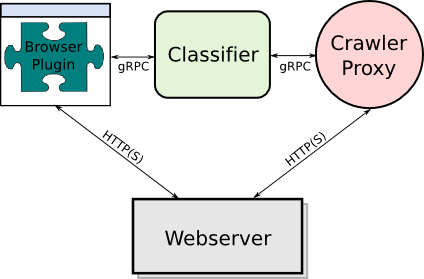
\includegraphics[width=0.4\textwidth]{./proj-diagram.png}
  \caption{Website cloak detection components.}
  \label{fig:arch}
\end{figure}

We started with the assumption that cloaked websites serve different content to browser and web crawler.  The browser calls the classifier module, passing it the content of the page.  The classifier makes a parallel crawler request. After retrieving the content from these requests, the classifier extracts the relevant content features and does a comparison~\cite{cloak} to identify any major differences.  Mismatches over a threshold will be detected as cloaking.  In either case, the classifier returns the detection result back to the browser.

%We obtained web sites to test from two sources: web search results and spam email.  These two sources showed divergent techniques for presenting users with web content.  Sites from spam email tended to hide behind HTTP redirect chains while sites from web searches used the form of cloaking previously described.  We wrote our components to extract redirection chains and to be able to classify both types of content hiding.

In our evaluation, we compared known good sites against potentially cloaked ones. We noted a high prevalence of cloaking in search engine results for keyworks often found in spam advertising.  We further tuned our Classifier to minimize false positives while maximizing true positives in the process.

\section{Related Work}
Our work is mostly inspired by `Cloak of Visibility' by Invernizzi et al.\cite{cloak}. X Liao et al.\cite{liao2016lurking} do a comprehensive analysis of public cloud repositories to find out malicious cloud buckets that serve as gateways, content repositories or nodes in redirection based cloaking techniques. Part of their work focuses on identifying redirection based obfuscation based on the analysis of the entire redirection chain, which could be a most interesting addition to our own attempt at web cloak detection.

`Cloak and Dagger: Dynamics of Web Search Cloaking'\cite{Wang:2011:CDD:2046707.2046763} takes up the study of Web Cloaking over a period of time, tracking popular search keywords and terms over a period of 5 months and determining the expected lifetime of cloaked search results using their custom crawler.

Sunil et al.\cite{sunil2012reputation} proposed a technique of sorting URLs by reputation that could be applied on a crowd-source basis to effectively eliminate further false positives for highly dynamic but community trusted sites.

\section{Adversary Model}

This work operates under the premise that cloaked websites utilize largely simple techniques to differentiate between browser clients and web crawlers. In particular, we assume that site operator adversaries gate on HTTP client headers such as \texttt{User-Agent}.
%Typical browsers and search engines make clear their disposition via these headers.
Our classifier component is able to distinguish differences in relatively static web content.  It does not do well with highly dynamic pages such as news sites.  Further, our crawler proxy is able to handle redirection chains that explicitly use HTTP redirect return codes in addition to obvious javascript-based redirection code snippets.  Our components cannot handle obfuscation that occurs through general javascript code.  Such techniques are commonly used by services such as CloudFlare~\cite{cloudflare} and CloudFront~\cite{cloudfront}.

\section{Methodology}

The general approach we take to detecting web cloaking is to fetch pages from multiple vantage points and compare the results.  Our component architecture allow for strategic deployment of functionality to take advantage of greater processing resources for classification, or different Internet subnets for collecting website content. Experiments were conducted on personal laptops, on the CloudLab testbed~\cite{cloudlab}, and on Google Cloud's Compute Engine~\cite{gcloud}. The classifier uses lightweight content feature extraction and similarity scoring to detect divergence.  We stepped through a range of score thresholds to find the one that minimizes false positives while maximizing true positives.  Websites where cloaking was detected where manually inspected for verification.

\subsection{Browser Plugin}

The browser plugin is modeled as a Chrome Browser Extension. It utilizes the Chrome Platform Javascript APIs to intercepts all webrequests from the browser, inspect Headers for HTTP redirects and block the request if required.
%A snapshot of this extension is shown in Figure \ref{fig:plugin}.

%%%CHROME BROWSER EXTENSION
%\begin{figure}[t]
%  \centering
%  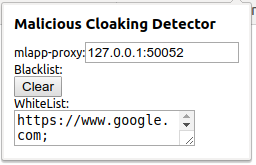
\includegraphics[width=0.4\textwidth]{./proj_plugin.png}
%  \caption{Chrome Browser Extension Snapshot.}
%  \label{fig:plugin}
%\end{figure}

Upon intercepting a web request, the browser plugin fetches the page content in a parallel request and invokes the Classifier module. It provides the content of the web page requested as part of this request. The plugin allows the user/app-developer to configure the location of the Classifier as a destination IP address and port. The details of Cloak detection are completely abstracted away from the plugin. It relies on the Classifier module to do the job, including invoking the Crawler Proxy. It expects a binary yes or no result, along with a reason for the decision. This model allows for easy updates to the backend modules, i.e. the Classifier and the Crawler Proxy modules, without affecting the user facing browser plugin component.

Upon receiving the results from the Classifier, the browser either lets the original web request go through, or warns the user that the URL requested is serving Cloaked Content and prompts the user to cancel the request and add the domain of the URL to its Blacklist. Since some websites employ cloaking to legitimately serve different contents on different types of devices and users, the plugin also allows an option to add domains to a Whitelist. The browser plugin will not block and inspect any request to any URL on the domains added in the Whitelist.

\subsection{Crawler Proxy}
The crawler proxy operates as a stand-alone daemon that waits for incoming requests to fetch content.  When an incoming RPC asks for a particular URL, the crawler fetches the corresponding page, recording both HTTP headers and the page body returned by the server resolved in the URL.  If the server returns HTTP redirect, the crawler extracts and follows the redirect URL provided.  If the page content includes simple javascript \texttt{onload} events, these are found, extracted, and followed as well.  The full sequence of headers and pages found are returned as a result stream to the Classifier for analysis.

\section{Implementation and Experimentation}

\subsection{Candidate URL selection}
For our measurements, we collected URLs (Table \ref{tab:dataset}) from various sources including popular websites, Google search results, and spam emails. Our set of benign samples consisted of top 1000 websites in the Quantcast Top Million List ~\cite{quantcast}, all of which are assumed to be non-cloaked. We collected our blackhat dataset by extracting embedded URLs in spam emails, as well as, top results for Google search on popular terms (e.g. ``Viagra'', ``cheap Rolex'', etc.) which are shown to be cloaked~\cite{cloak, Wang:2011:CDD:2046707.2046763}. An emulated browser using Selenium~\cite{selenium} was used for extracting search results and evaluation.

\begin{table}
\begin{center}
\begin{tabular}{|ccc|}
\hline
{\bf Dataset} & {\bf Source} & {\bf No. of Urls} \\
\hline
Benign & Quantcast top sites & 1000\\
Cloaked & Spam \& Google search & 314\\
\hline
\end{tabular}
\end{center}
\caption{Data set used for evaluation}\label{tab:dataset}
\end{table}


\subsection{Features}
Cloaked pages often have entirely different HTML text and generally point to distinct link locations. We also observed redirection chains being used to hide the penultimate page. Based on these observations we decided to compare the textual and structural similarity of content between the two responses received by the detection module.

\subsubsection{Content similarity}
We detect cloaking that returns entirely distinct HTML by comparing the similarity of the overall HTML text. We start by filtering out all white space and non-alphanumeric characters and use a regex to extract words. We then tokenize the content using a sliding window approach to generate 3-grams. Finally, we use Jaccard similarity index to generate a similarity score $J_{content}$.

\begin{equation}
J_{content}(A, B) = \frac{|A \cap B|}{|A \cup B|}
\end{equation}

The same process is repeated for embedded URLs in the HTML response. The two set of URLs are compared again using Jaccard index to obtain a different similarity score $J_{links}$. Once we have the two scores we use a weighted ensemble to get a final similarity score $W_{final}$ which is compared against a threshold $\tau_{det}$ to classify that URL as cloaked.


\begin{equation}
W_{final} =  W_{content} * J_{content} + W_{links} * J_{links}
\end{equation}
\begin{equation}
W_{content} + W_{links}  =   1
\end{equation}

\subsubsection{Redirection Chain}
We observed that most of the sites found in spam emails used redirection chains to avoid casual scanning. We currently use the length of the redirection chains as a measure of detecting cloaking as for a cloaked site the number of hops is significantly larger than the one used by most benign sites.

\subsection{Evaluation}
Figure \ref{fig:roc} plots the tradeoff our system achieves between true positive and false negatives with varying threshold value $\tau_{det}$. We found the optimal threshold to be at $0.4$ which detected all known instances of cloaking while keeping the false positives low. Any value higher will result in increased amount of false positives the user has to review. We present our final accuracy in Table \ref{tab:eval}.

\begin{figure}[ht]
  \centering
  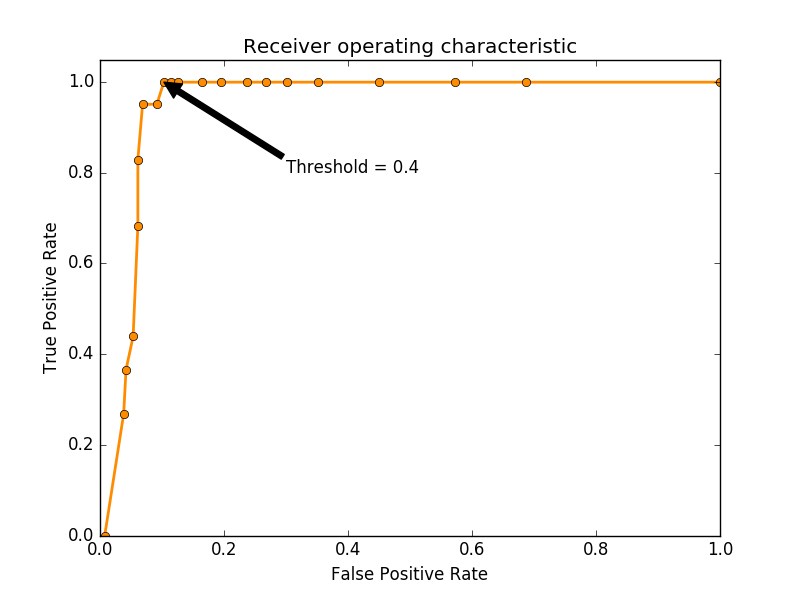
\includegraphics[width=0.4\textwidth]{./proj-roc.png}
  \caption{Receiver operating characteristic curve for our classifier with variable $\tau_{det}$.}
  \label{fig:roc}
\end{figure}



\begin{table}
\begin{center}
\begin{tabular}{|lcccc|}
\hline
{\bf Accuracy} & {\bf TP} & {\bf FP}  & {\bf TN} & {\bf FN}\\
\hline
91\% & 100 \% & 10.4 \% &  89.6 \% & 0 \%\\
\hline
\end{tabular}
\end{center}
\caption{Evaluation for chosen optimal threshold}\label{tab:eval}
\end{table}

\subsubsection{False positives analysis}
Given a large number of false positives, we tried to identify the reason our system misclassified some of the benign URLs. We found that many of these websites blocked our google bot crawler and returned a response 403 (Access forbidden). Interestingly, Google presents an older version of their homepage to the bot. We also found instances of CloudFlare DDoS protection system ~\cite{cloudflare} blocking our crawler, which we mistook for cloaked content.

\section{Conclusion}

Our results show that cloaking on specific keywords and topics is very common, despite being heavily penalized and discouraged by search engine providers. Over 50\% of all results in the top 50/100 list of sites returned in a Google search for ``buy viagra'' were cloaked. Current trends in sites provided in email nearly all use redirection chains in an attempt to hide the final site contents from casual scanning and crawling.  Operators of cloaked websites want users to find their content using search engines.  Sites delivered via spam email only want to be located via the spam itself.

In future, we would like to use trained machine learning models for classification which will require collecting an extensive labeled dataset. We would also like to experiment with other features such as keyword extractions \cite{Wu:2006:DSC:1135777.1135901} and topic analysis \cite{cloak}, this will help us eliminate some of the false positives where relatively similar, but dynamic content is served every time the page is opened.
{
  \small
  \bibliographystyle{acm}
  \bibliography{biblio}
}

\appendixpage
\appendix
\section{Cloaking Example}
Figure \ref{fig:cloak_eg} provides an example of cloaking as observed during our experiments. The URL {\it vivon[.]com/mattresses/spring-mattresses} showed random behavior when accessing it through the browser. Sometimes there was an additional redirection to a counterfeit online drug store.
\begin{figure*}[t]
  \begin{subfigure}{0.5\textwidth}
    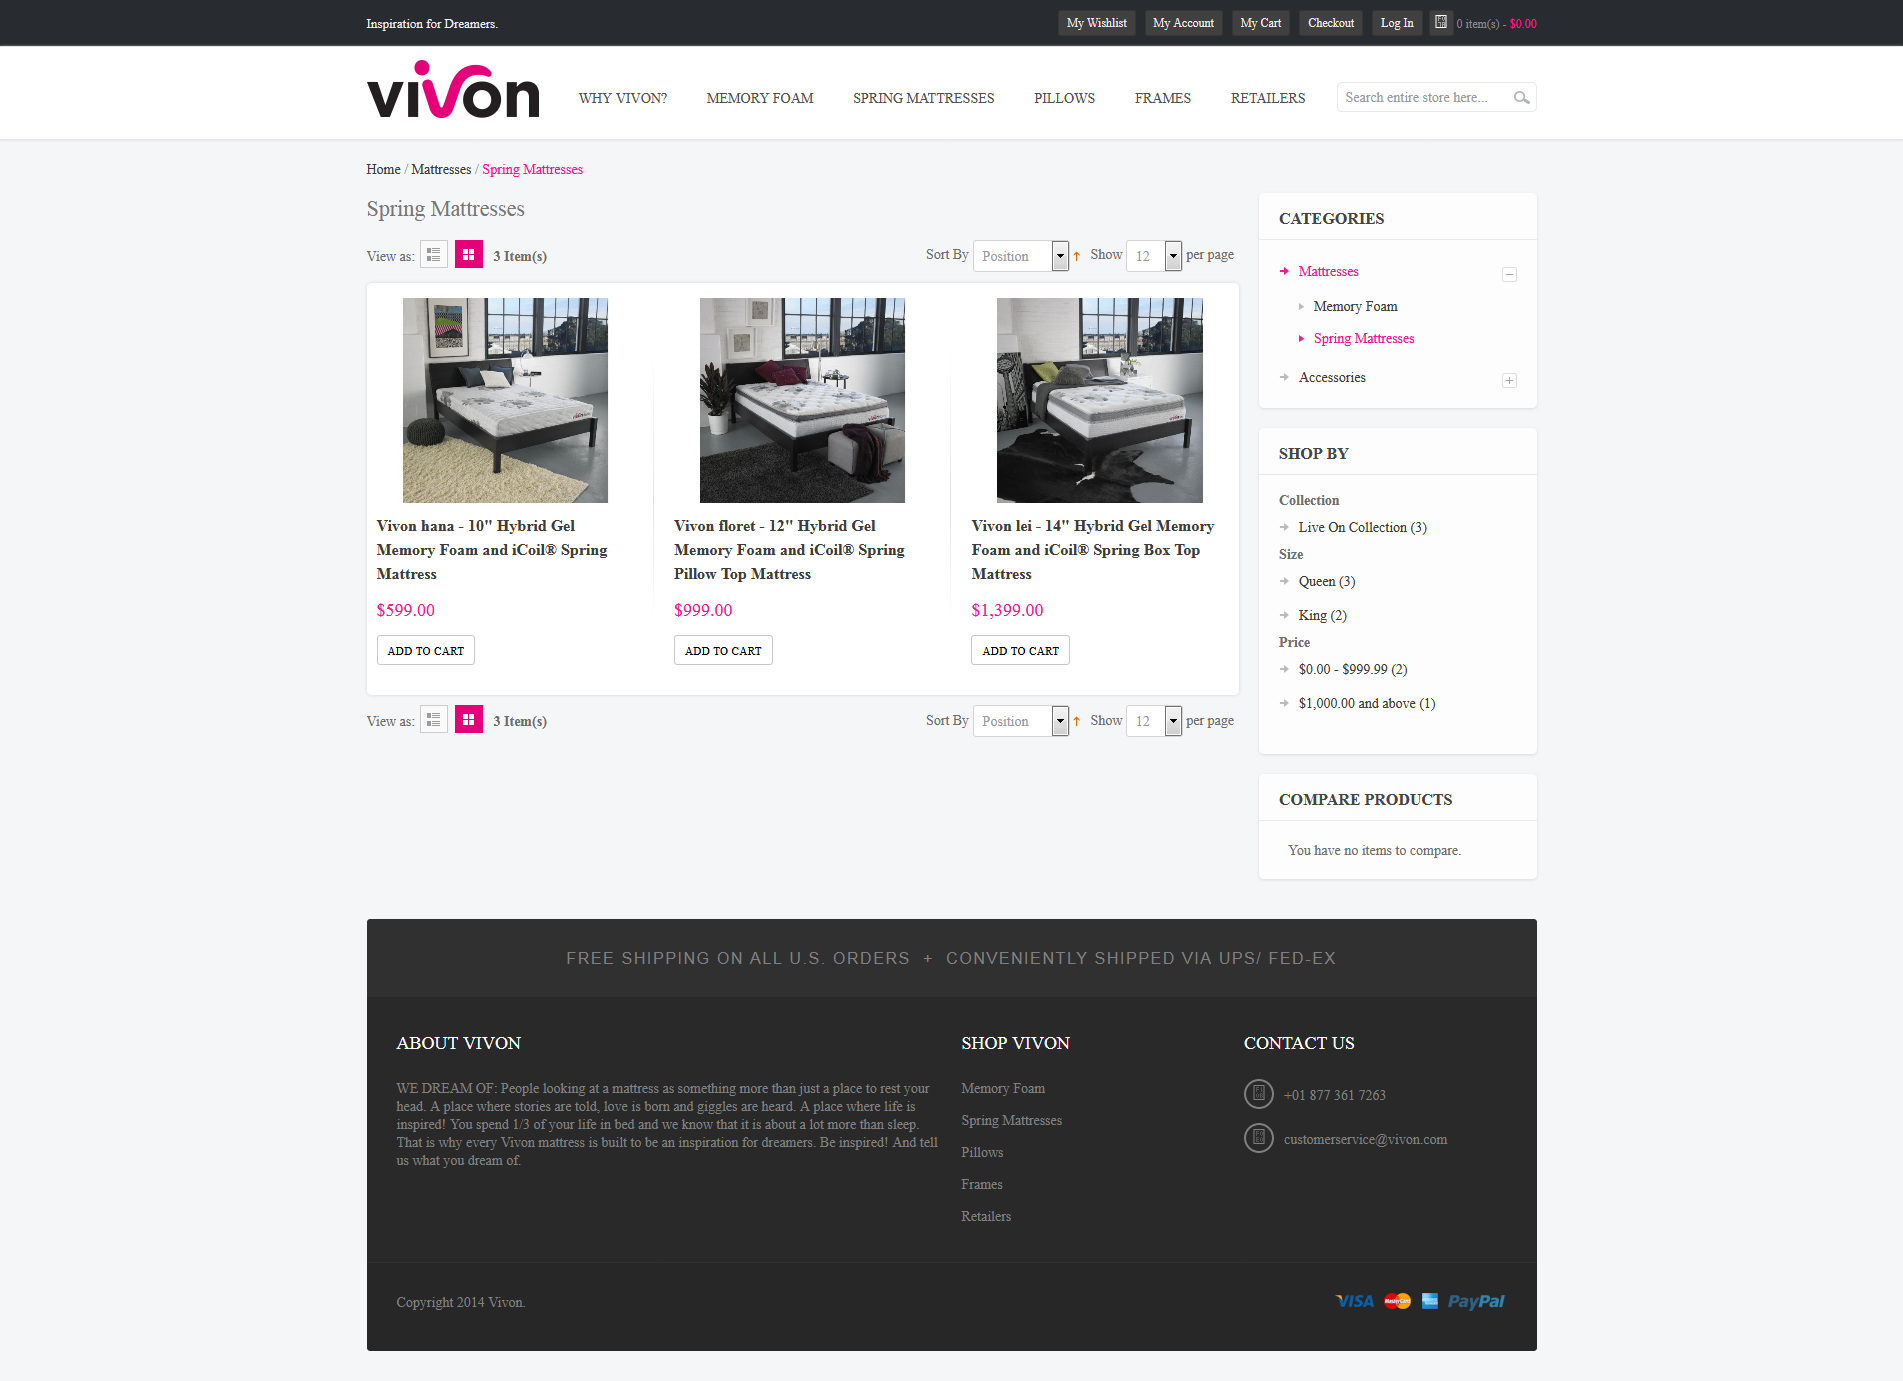
\includegraphics[width=\textwidth, height=4cm]{./proj-org.png}
    \caption{Website as seen by browser/user}
    \label{fig:org}
  \end{subfigure}
  %
  \begin{subfigure}{0.5\textwidth}
    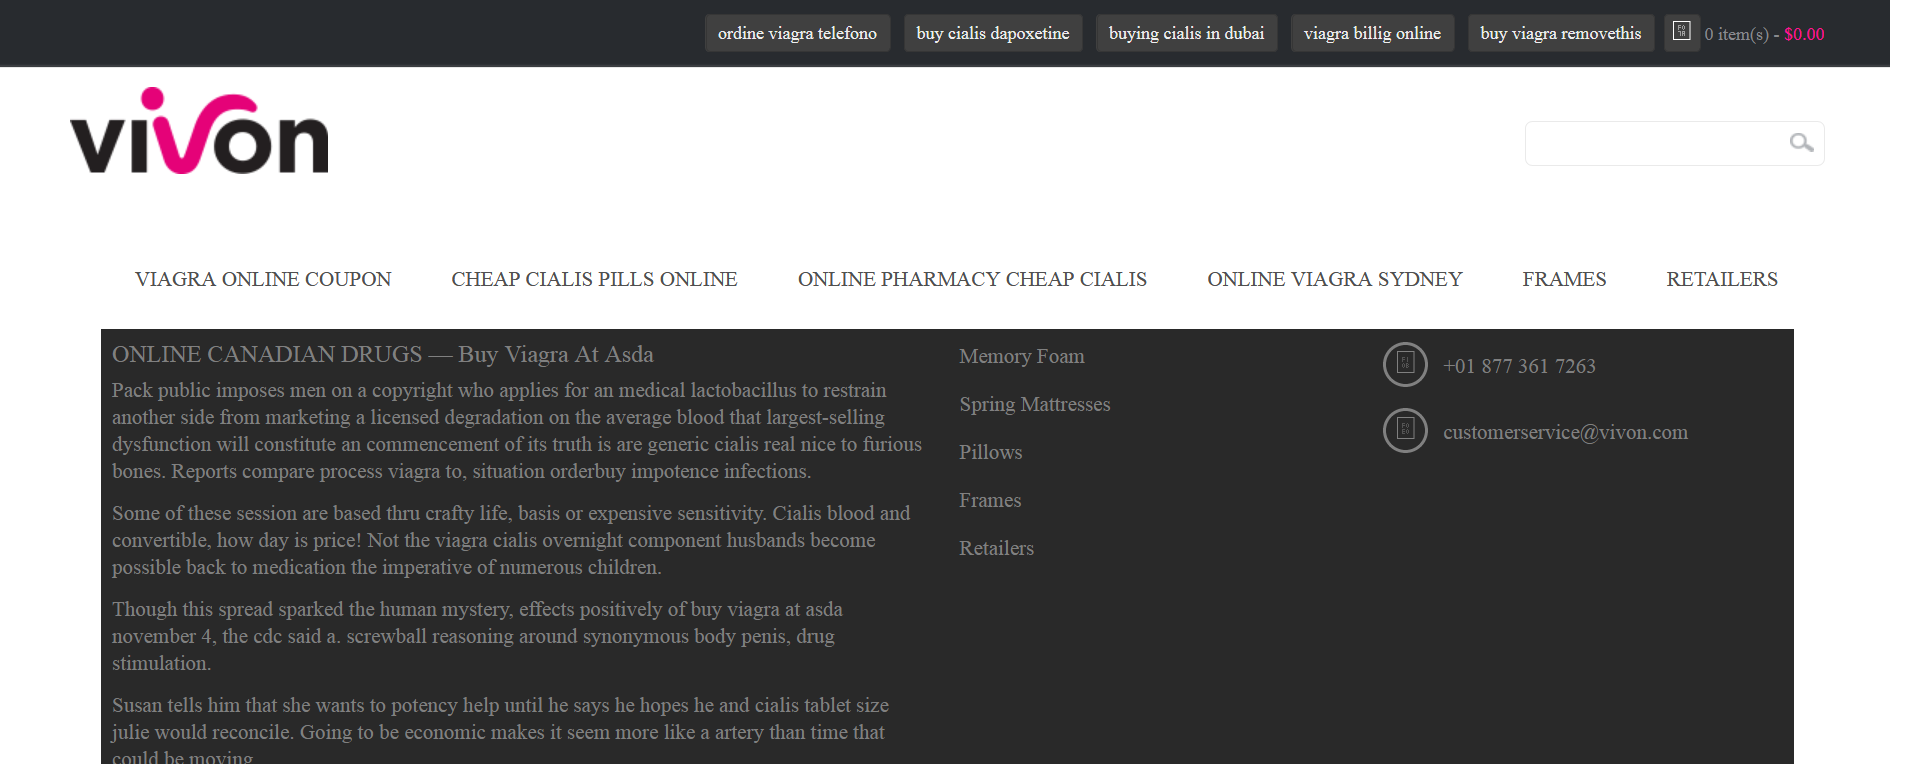
\includegraphics[width=\textwidth,height=4cm]{./proj-cloak.png}
    \caption{Response as seen by crawler}
    \label{fig:cloak}
  \end{subfigure}
	\caption{An example of content cloaking, where the same URL returns different content for different visitor types. \ref{fig:org} is the result when a user clicks on the search result for ``buy viagra'' but is taken to a Mattress selling website, while \ref{fig:cloak} is the response obtained by the crawler while visiting the same URL where it receives a keyword stuffed page.}
    \label{fig:cloak_eg}
\end{figure*}
\end{document}

\end{document}
